85. а) $y=\cfrac{x^2-3x}{3-x}+1=\cfrac{x(x-3)}{3-x}+1=\begin{cases} 1-x,\\ x
eq 3.\end{cases}$\\
\begin{figure}[ht!]
\center{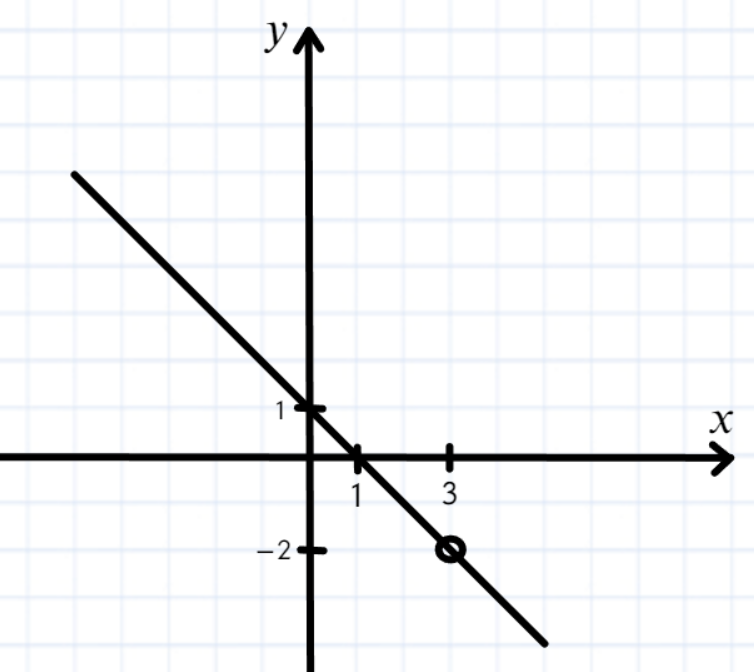
\includegraphics[scale=0.35]{gr7-85.png}}
\end{figure}\\
б) При положительных $x$ функция принимает значения $(-\infty;-2)\cup(-2;1).$\\
в) Эта прямая не будет иметь общих точек с графиком функции, если она параллельна прямой $y=1-x$ или если она проходит через выколотую точку $(3;-2).$ Пусть это прямая $y=kx+b.$ В первом случае её угловой коэффициент равен $-1,$ значит $-1=2+b,\ b=-3,$ то есть это функция $y=-x-3.$ Во втором случае $\begin{cases} -2=3k+b,\\ -1=-2k+b.\end{cases}\Leftrightarrow
\begin{cases} -1=5k,\\ b=2k-1.\end{cases}\Leftrightarrow
\begin{cases} k=-\cfrac{1}{5},\\ b=-\cfrac{7}{5}.\end{cases},$ то есть прямая задана уравнением $y=-\cfrac{1}{5}x-\cfrac{7}{5}.$\\
